\documentclass[12pt, a4paper]{article}
\usepackage[utf8]{inputenc}
\usepackage{amssymb}
\usepackage{indentfirst}
\usepackage{listings}
\usepackage{enumitem}
\usepackage{comment}
\usepackage{graphicx}
\usepackage{color}
\usepackage[portuguese]{babel}
\usepackage{geometry}
\geometry{legalpaper, a4paper,
 total={170mm,257mm},
 left=20mm,
 top=20mm}
\setlength{\voffset}{-10mm}
\definecolor{dkgreen}{rgb}{0,0.6,0}
\definecolor{gray}{rgb}{0.5,0.5,0.5}
\definecolor{mauve}{rgb}{0.58,0,0.82}

\lstset{frame=tb,
  language=Java,
  aboveskip=3mm,
  belowskip=3mm,
  showstringspaces=false,
  columns=flexible,
  basicstyle={\small\ttfamily},
  numbers=none,
  numberstyle=\tiny\color{gray},
  keywordstyle=\color{blue},
  commentstyle=\color{dkgreen},
  stringstyle=\color{mauve},
  breaklines=true,
  breakatwhitespace=true,
  tabsize=3
}

\newcommand{\tit}[1]{\textit{#1}}
\newcommand{\tb}[1]{\textbf{#1}}
\newcommand{\tbi}[1]{\textbf{\textit{#1}}}

\newcommand{\bitem}[2]{ \tb{(\tit{#1}) {#2}}}
\newcommand{\iitem}[1]{(\tit{#1})}

\newcommand{\oo}{orientação à objetos}
\newcommand{\sw}{\tit{software}}
\newcommand{\ssw}{\tit{software} }

\newcommand{\question}[1]{\item \tb{#1}}
\newcommand{\answer}[1]{\par \tb{Resposta:} #1}

\newcommand{\quotes}[1]{``#1''}

\title{Módulo 3 - Atividade Individual \\
  \large Engenharia de Requisitos}

\author{Wellington M. Espindula}
\date{Fevereiro de 2021}

\begin{document}
    \maketitle
    
    \begin{enumerate}[label=\textbf{\arabic*.}]
        % Question 1
        \question{Considere a seguinte descrição de um sistema: “A cafeteira tem uma luz vermelha que pisca quando está ligada, quando a água chega na temperatura certa ela fica ligada (sem piscar)” Quais seriam os “reais” requisitos?}
        \answer{ \\ \\
            Requisitos:
            \begin{itemize}
                \item RF - A cafeteira deve passar café.
                \item RF - A cafeteira deve deve aquecer a água para passar o café.
                \item RNF - A cafeteira deve piscar a LED vermelha assim que estiver ligada e aquecendo a água.
                \item RF - A cafeteira deve desligar o aquecimento da água quando a temperatura certa for atingida.
                \item RNF - A cafeteira deve manter a LED constante assim que a temperatura correta for atingida.
                \item RF - A cafeteira deve manter o café quente após a água ter sido aquecida.
            \end{itemize}
        } \newpage
        
        % Question 2
        \question{Casos de Uso – Loja de CDs. Faça o diagrama de casos de uso do seguinte enunciado. \\
            \normalfont{\tit {
            Uma loja de CDs possui discos para venda. Um cliente pode comprar uma quantidade ilimitada de discos para isto ele deve se dirigir à loja. A loja possui um atendente cuja função é atender os clientes durante a venda dos discos. A loja também possui um gerente cuja função é administrar o estoque para que não faltem discos. Além disso é ele quem dá folga ao atendente, ou seja, ele também atende os clientes durante a venda dos discos. \\ \\
            As vendas podem ser à vista ou a prazo. Em ambos os casos o estoque é atualizado e uma nota fiscal, entregue ao consumidor. \\ \\
            No caso de uma venda à vista, clientes cadastrados na loja e que compram mais de 5 CDs de uma só vez ganham um desconto de 1\% para cada ano de cadastro. \\ \\
            No caso de uma venda a prazo, ela pode ser parcelada em 2 pagamentos com um acréscimo de 20\%. As vendas a prazo podem ser pagas no cartão ou no boleto. Para pagamento com boleto, são gerados boletos bancários que são entregues ao cliente e armazenados no sistema para lançamento posterior no caixa. Para pagamento com cartão, os clientes com mais de 10 anos de cadastro na loja ganham o mesmo desconto das compras a vista. \\ \\ 
            Para efetuar vendas ou administrar estoque, atendentes e gerentes terão que validar suas respectivas senhas de acesso ao sistema.
            }}
        }
        \answer{
           \begin{figure}[ht!]
               \centering
               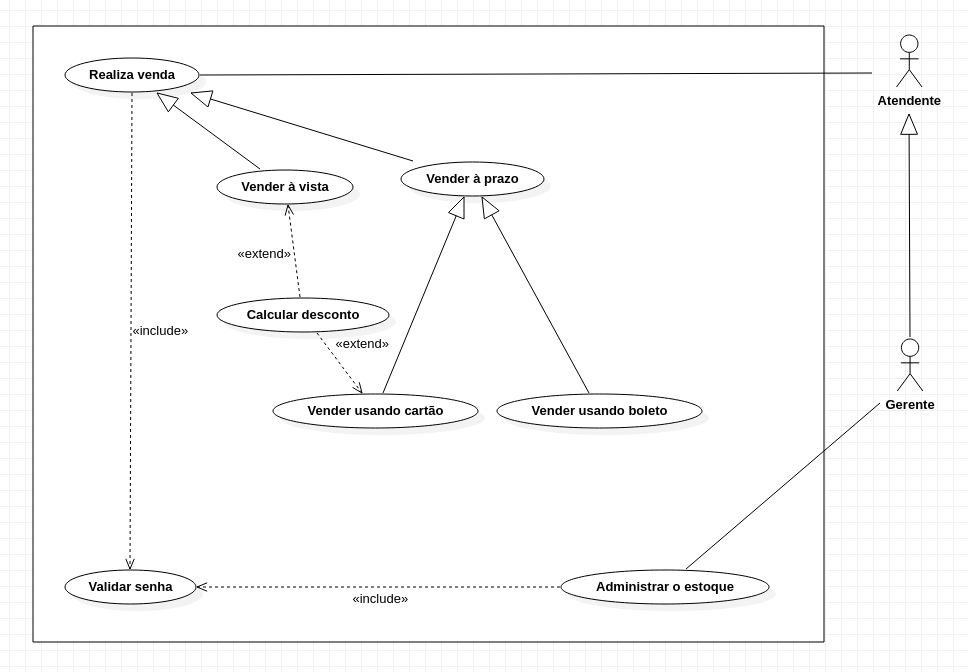
\includegraphics[height=0.45\textheight]{quest2_1.png}
               \label{fig:quest2}
               \caption{Diagrama de Caso de Uso da Loja de CDs. Fonte: O Autor, 2021.}
           \end{figure} 
        } \newpage
        
        % Question 3
        \question{
            Um software que visa auxiliar no gerenciamento de um hospital público de assistência pré-natal precisa ser desenvolvido, e ele consiste das seguintes principais funcionalidades: 
            \normalfont{
                \begin{enumerate}[label={\alph*.}]
                    \item Cadastro de pacientes em geral e particularidades de gestantes e gestação, para gestante que realizaram e/ou estão realizando acompanhamento pré-natal;
                    \item Agendamento de consultas pré-natal;
                    \item Realização de consultas pré-natal;
                    \item Verificação do seguimento, pelos médicos e enfermeiras, de protocolos estabelecidos pelo governo no atendimento pré-natal; e 
                    \item Cadastro, alteração e exclusão de protocolos relacionados com a assistência pré-natal.
                \end{enumerate}
            }
            Faça o diagrama de casos de uso deste sistema. Após isto, responda o que deve ser alterado no diagrama caso:
            \normalfont{
                \begin{enumerate}[label={\alph*.}]
                    \item Membros da equipe médica também pudessem manter pacientes e agenda consultas?
                    \item As consultas possuam uma certa interação com o Sistema em comum, mas existe uma diferenciação entre a primeira consulta e as demais?
                \end{enumerate}
            }
        }
        \answer{
           \begin{figure}[ht!]
               \centering
               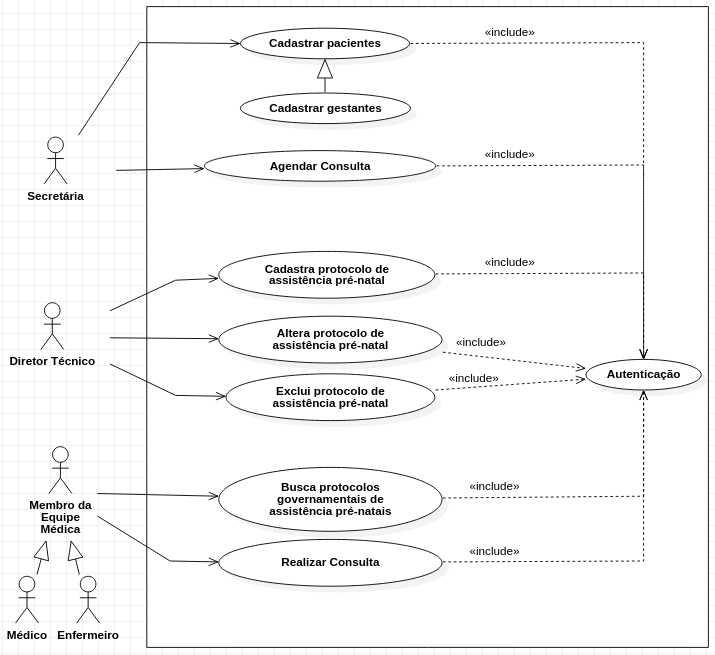
\includegraphics[width=0.85\textwidth]{quest3_1.png}
               \caption{Diagrama de Casos de Uso do \ssw pré-natal. Fonte: O Autor, 2021.}
               \label{fig:quest31}
           \end{figure}
           
           Para a alteração proposta no item \tb{a.}, o diagrama deve ser alterado adicionando uma relação entre médicos e agendar consulta, bem como deve ser adicionado um caso de uso chamado de Desagendar Consulta e outro complementar chamado Manter Consulta, caso de uso cujo médico deveria ser relacionado com. Para o item \tb{b.}, o caso de uso Agendar Consulta deveria ser especializado para o Caso de Uso Agendar Primeira Consulta. As alterações propostas podem ser visualizadas na imagem \ref{fig:quest32}.
           \begin{figure}[ht!]
               \centering
               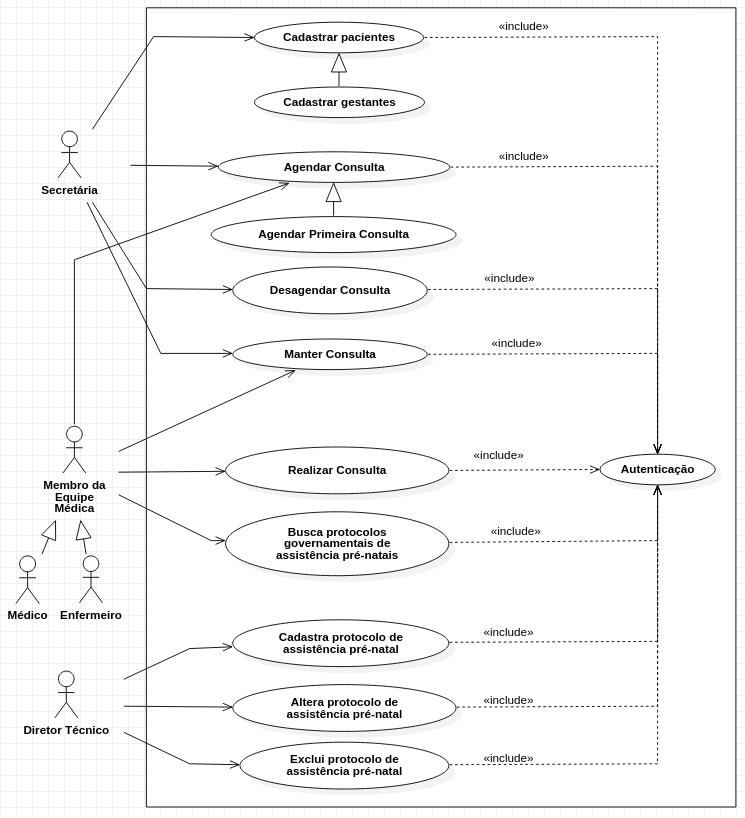
\includegraphics[width=0.92\textwidth]{quest3_2.png}
               \caption{Diagrama de Casos de Uso do \ssw pré natal após novas alterações. Fonte: O Autor, 2021.}
               \label{fig:quest32}
           \end{figure}
           
        }
        \newpage
        
        % Question 4
        \question{Considere o sistema de assistência pré-natal descrito na pergunta anterior, e os documentos “Modulo 3 - SUAP - Observação.pdf” e “Modulo 3 - SUAP - Documentação.pdf” fornecidos no moodle. Com base neles, faça a descrição do caso de uso “Realizar Consulta”}
        \answer{ \\
           \fbox{
                \parbox{0.91\textwidth}{
                    \tb{Identificação:} Realizar Consulta \\
                    \tb{Ator:} Médico ou Enfermeiro \\
                    \tb{Descrição:} Permite ao médico/enfermeiro armazenar os dados da consulta - em uma espécie de laudo, informando, por exemplo, o peso, altura, IMC e pressão arterial do paciente -, uma vez que o médico ou o enfermeiro esteja autenticado no sistema e o paciente esteja cadastrado e possuir a consulta agendada. Desse modo, as informações do paciente devem ser atualizados no sistema. \\ 
                    \tb{Pré-Condições:} O paciente deve possuir uma consulta agendada anteriormente e o Médico deve estar autenticado no \sw. \\
                    \tb{Pós-Condições:} Os dados da consulta são inseridos no \sw \\ \\ 
                    
                    \tb{Seção Principal} \\
                     \begin{enumerate}[label={\arabic*.}]
                         \item O médico/enfermeiro autentica-se no sistema informando seu \tit{login} e \tit{senha}.
                         \item O sistema verifica se o usuário é válido e se a senha está em conformidade à cadastrada.
                         \item 
                         \begin{enumerate}[label={\alph*.}]
                             \item Se o usuário ou senha estiver incorreta, informa ao usuário que os dados estão incorretos.
                             \item Se o usuário ou senha estiver correta, autoriza acesso ao sistema.
                         \end{enumerate}
                         \item O médico/enfermeiro realiza a consulta o paciente.
                         \item Tendo em vista as informações mensuradas do paciente (como peso, altura e pressão arterial) dentre outros dados relevantes, o médico/enfermeiro deverá inseri-las no sistema preenchendo a ficha de consulta.
                         \item O sistema deverá guardar as informações da consulta.
                     \end{enumerate}
                    
                }
            }
        }
        \newpage
        
        
        % Question 5
        \question{Faça a descrição de um caso de uso de log in em um sistema onde o usuário deve fornecer seu nome de usuário e senha e, caso eles sejam válidos, o sistema deve autenticar o usuário. Caso contrário deve bloquear a autenticação. Não se esqueça que a descrição de um caso de uso deve ser completa e precisa.}
        \answer{ \\ \\
            \tb{Identificação:} \tit{Login} \\
            \tb{Ator:} Usuário do sistema \\
            \tb{Descrição:} Verifica se o usuário é autêntico verificando se os dados de nome de usuário e senha estão em conformidades aos previamente cadastrados no sistema e oferecendo suporte a recuperação de acesso à conta. \\ 
            \tb{Pré-Condições:} O usuário previamente ter uma conta cadastrada no sistema. \\
            \tb{Pós-Condições:} Libera acesso ao sistema, concedendo ao dispositivo utilizado pelo usuário (por exemplo, navegador \tit{web} ou aplicativo) uma sessão de tempo finito de acesso ao sistema. \\
            
            \tb{Seção Principal}
             \begin{enumerate}[label={\arabic*.}]
                 \item O usuário informa ao sistema seu nome de usuário e senha, confirmando o envio do formulário.
                 \item O sistema verifica se o usuário está cadastrado no seu banco de dados.
                     \begin{enumerate}[label={\alph*.}]
                         \item Se o usuário foi encontrado, verifica se o código \tit{hash} da senha informada é igual ao código \tit{hash} da senha consistida no banco de dados.
                            \begin{enumerate}[label={\roman*.}]
                                 \item Se os códigos de codificação das senhas forem iguais, autoriza o acesso ao sistema, abrindo uma nova sessão para o usuário e redirecionando-o para a tela principal do sistema .
                                 
                                 \item Caso os códigos das senhas forem diferentes, retorna à tela de login informando a mensagem \quotes{A senha está incorreta!} escrita em vermelho.
                            \end{enumerate}
                         
                         \item Se o usuário não foi encontrado, retorna à tela de login informando a mensagem \quotes{O usuário informado não existe!} escrita em vermelho.
                     \end{enumerate}
                 \item Caso a autenticação tenha sido mal-sucedida e tenha retornado à página inicial, exiba a mensagem de erro.
                 \item Atualize a contagem de tentativas de \tit{login}, incrementando-a.
                 \item Dispare uma tarefa na aplicação cliente de \tit{login} que inative o \tit{login} por $ 100 \cdot 4^n $ ms, sendo $n$ o número de tentativas de \tit{login}.
                 \item Exiba uma caixa perguntando se o usuário esqueceu a senha.
                 \begin{enumerate}[label={\alph*.}]
                     \item Caso o usuário tenha esquecido a senha, exibe a tela de esqueci minha senha.
                     \begin{enumerate}[label={\roman*.}]
                         \item O usuário insere ao sistema o seu e-mail e confirma o envio do formulário.
                         \item O sistema envia um e-mail ao endereço do usuário cadastrado com um \tit{link} de mudança de senha.
                         \item Ao entrar no \tit{link} enviado por e-mail, o usuário informa a nova senha em duplicata.
                         \item O sistema checa se senhas são iguais entre si.
                         \begin{itemize}
                             \item Caso sejam, o sistema atualiza a senha do usuário no banco de dados, salvando apenas a \tit{hash} da mesma.
                             \item Caso contrário, o sistema retorna ao usuário uma mensagem de erro afirmando que as senhas não coincidem e retorna à página de cadastro da nova senha
                         \end{itemize}
                     \end{enumerate}
                 \end{enumerate}
                \item O usuário informa novamente o nome de usuário e senha e confirma o envio do formulário.
                \item O sistema verifica se o número de tentativas $n$ é maior que 10.
                    \begin{enumerate}
                         \item Caso o usuário tenha extrapolado o número de tentativas $n>10$. Bloqueia o acesso do sistema pelo o dispositivo utilizado.
                         \item Caso contrário, retorna à etapa 2 (validação de usuário e senha).
                     \end{enumerate}
             \end{enumerate}
        }
        \newpage
 
    
        % Question 6
        \question{Considere o enunciado “Modulo 3 - Biblioteca – Enunciado.pdf” fornecido no moodle. Com base nele, faça o diagrama de casos de uso do sistema e a descrição do caso de uso “Efetuar Empréstimo”}
        \answer{ \\ \\
          \tb{Diagrama de casos de Uso:}\\
          \begin{figure}[ht!]
               \centering
               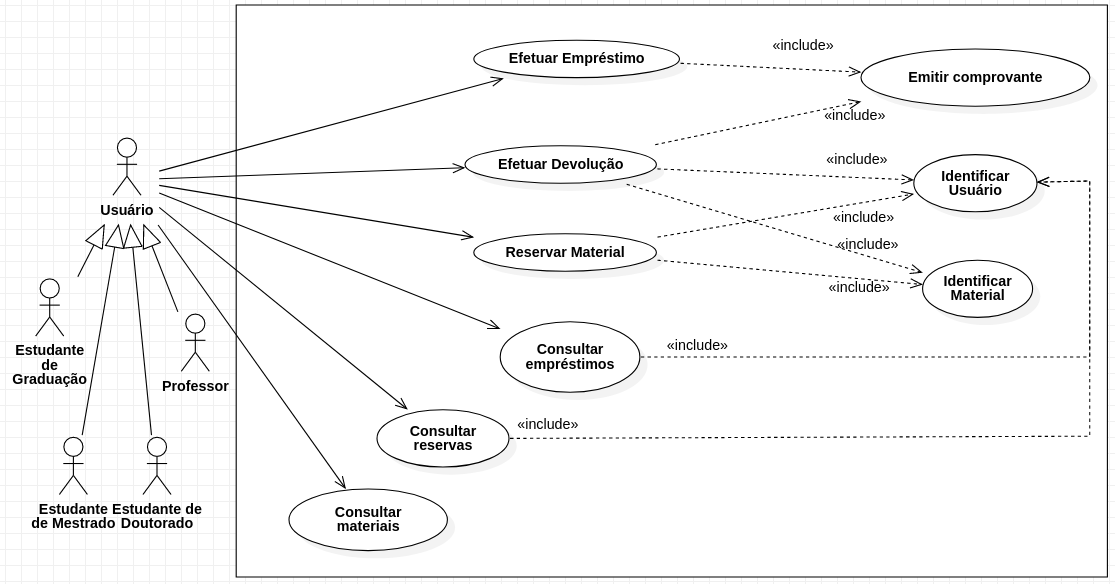
\includegraphics[width=0.92\textwidth]{quest6.png}
               \caption{Diagrama de Casos de Uso do \ssw do Sistema de Biblioteca. Fonte: O Autor, 2021.}
               \label{fig:quest6}
           \end{figure}
           
           Segue na próxima página a descrição de casos de uso.
            
            \fbox{
                \parbox{0.91\textwidth}{
                    \tb{Descrição de caso de Uso:} \\ \\
                    \tb{Identificação:} Efetuar empréstimo \\
                    \tb{Ator:} Usuário \\
                    \tb{Descrição:} Permite usuário efetuar o empréstimo de um material da biblioteca tendo em vista as restrições de empréstimo. \\ 
                    \tb{Pré-Condições:} O usuário deve ser aluno de Graduação, Pós-Graduação (Mestrando ou Doutorando) ou Professor \\
                    \tb{Pós-Condições:} O empréstimo deverá ser realizado e o comprovante de empréstimo deverá ser emitido \\
                    
                    \tb{Seção Principal}
                     \begin{enumerate}[label={\arabic*.}]
                         \item O usuário deve selecionar seu nome na lista de usuários.
                         \item O usuário deve selecionar o material escolhido e realizar a operação de empréstimo.
                         \item Verifica se existe algum exemplar do material disponível.
                         \begin{enumerate}[label={\alph*.}]
                             \item Caso não exista, exibe a mensagem \quotes{Não existe exemplar disponível para empréstimo} para o usuário.
                         \end{enumerate}
                         \item Verifica se não há pendências do usuário.
                         \begin{enumerate}[label={\alph*.}]
                             \item Caso haja, exibe a mensagem \quotes{Você tem empréstimos atrasados} para o usuário.
                         \end{enumerate}
                         \item Verifica se o usuário não atingiu seu limite de empréstimos.
                         \begin{enumerate}[label={\alph*.}]
                             \item Caso tenha atingido, exibe a mensagem \quotes{Você atingiu seu limite de empréstimos} para o usuário.
                         \end{enumerate}
                         \item Verifica se a quantidade de reservas do material é menor do que a quantidade de exemplares disponíveis.
                         \begin{enumerate}[label={\alph*.}]
                             \item Caso seja, exibe a mensagem \quotes{Os exemplares deste material já se encontram reservados} para o usuário.
                         \end{enumerate}
                         \item Verifica se o usuário já havia realizado o empréstimo deste mesmo material.
                         \begin{enumerate}[label={\alph*.}]
                             \item Caso seja, exibe a mensagem \quotes{Você já realizou o empréstimo desse material} para o usuário.
                         \end{enumerate}
                         \item \tit{Include} Emitir comprovante.
                     \end{enumerate}
                     
                     \tb{Requisitos Não-Funcionais}
                     \begin{itemize}
                         \item As respostas do sistema devem demorar no máximo 10 segundos.
                         \item A interface gráfica deve ser acessível à alunos com deficiência visual.
                     \end{itemize}
             }}
        }
        
    \end{enumerate}



    
\end{document}